\chapter{Ethereum: Sviluppo di applicazioni decentralizzate}
\label{ch:ethereum}

Seguendo la divisione in tre strati di concetti, implementazioni e istanze, definita fin dall'inizio del lavoro, in questo capitolo verrà affrontato l'aspetto implementativo, nel caso concreto della piattaforma Ethereum. I concetti spiegati fino a questo punto possono costituire una base decisionale, un punto di partenza per scegliere le implementazioni che meglio si adattano alle proprie necessità. Possono essere visti come una sorta di contenitore aperto da cui è possibile “pescare” le componenti concettuali da implementare con i relativi pro e contro a seconda degli obiettivi delle applicazioni finali. 

Importante sottolineare che lo stato dell'arte delle blockchain limita l’utilità di descrivere in dettaglio un certo numero di implementazioni concrete. Questa affermazione deriva dal contesto attuale, le blockchain nonostante non siano più definibili come una tecnologia fra le più recenti in confronto alle tempistiche del settore informatico, generalmente non hanno raggiunto una stabilità sufficiente. Usando la terminologia presente nelle analisi e predizioni annuali condotte dalla Gartner\footnote{Gartner è una società di consulenza nel campo dell'Information Technology. Effettua analisi e ricerche al fine di produrre previsioni attendibili per i vari processi decisionali e di investimento.} la blockchain si trova attualmente sulla via di uscita dal cosiddetto "\emph{hype cycle}"\footfullcite{gart2016} \smallskip \footfullcite{gart2018}. Una metodologia usata per rappresentare la maturità, l'adozione e l'applicazione di nuove tecnologie.

\begin{figure}[H]
\centering
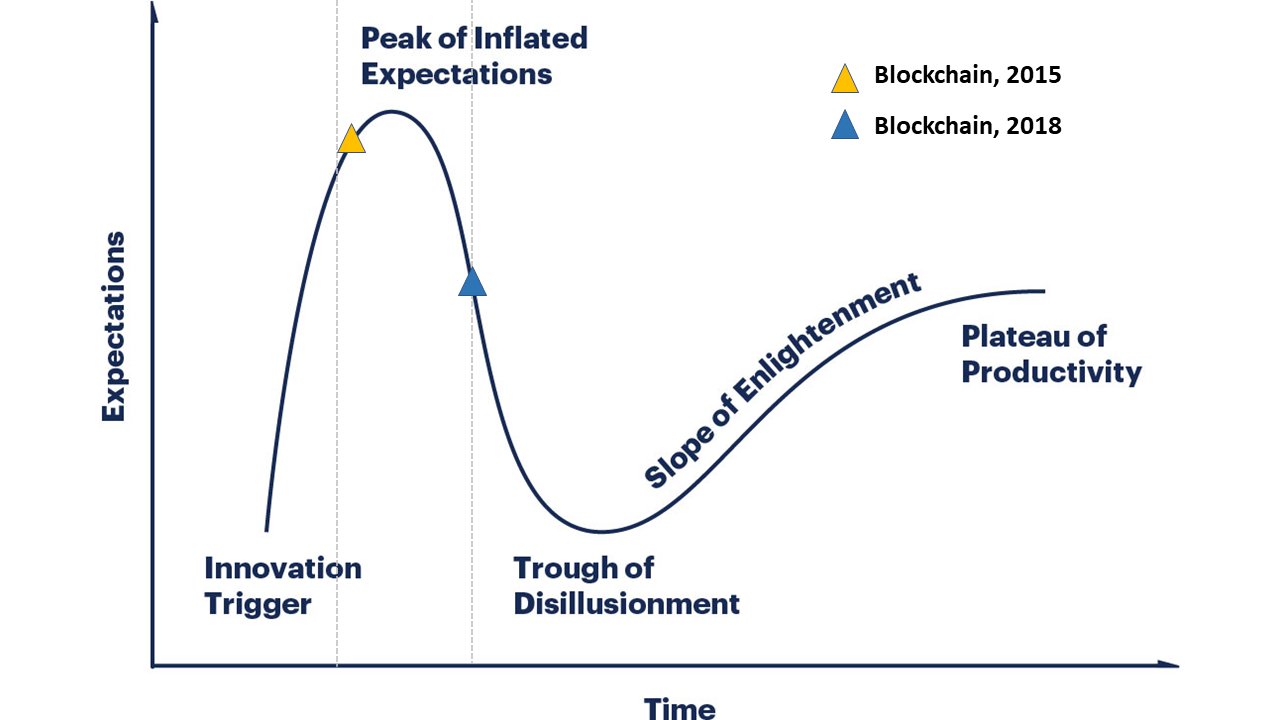
\includegraphics[width=1\textwidth]{immagini/blockchainHype.png}
\caption{Tecnologia blockchain: Hype Cycle}
\label{fig:HypeCycleBlockchain}
\end{figure}

La situazione in figura \ref{fig:HypeCycleBlockchain}, può essere vista come un contesto variabile, di continuo sviluppo con l’emergere di nuove implementazioni, piattaforme e applicazioni. Si tratta di una ricerca spesso finalizzata al miglioramento e all'adozione delle nuove tecniche per contrastare le limitazioni attuali del paradigma blockchain, in una situazione, qual è quella presente, in continuo mutamento e caratterizzata dall'instabilità e in alcuni casi da cambiamenti radicali. Tuttavia, questo non pregiudica l’utilità delle cose dette finora in quanto si tratta di concetti fondamentali che, nel caso peggiore, possono servire anche per comprendere le scelte e gli sviluppi futuri della tecnologia.

La scelta di Ethereum come sistema da presentare, collegato alla successiva costruzione di un’applicazione nel capitolo successivo è stata fatta seguendo tra le altre, queste motivazioni di stabilità, di sviluppo e di innovazione. Viene perseguita l'idea legata alla correlazione tra il successo e la popolarità di un sistema, misurata tenendo conto del numero di partecipanti e di sviluppatori coinvolti, degli strumenti di sviluppo messi a disposizione e dal loro grado di maturità. Si è tenuto conto, anche della frequenza di aggiornamenti e dell’interesse della comunità, degli enti pubblici e privati con i relativi rischi connessi. Un insieme di fattori che le nuove implementazioni dovranno cercare di raggiungere per attrarre nuovi utenti e sviluppatori ai loro sistemi. Al momento dello scrivere la piattaforma Ethereum è il sistema più sviluppato sotto questi aspetti anche grazie all'integrazione di strumenti per la costruzione di applicazioni decentralizzate.

\section{Implementazione Ethereum}

Ethereum è una piattaforma di sviluppo delle applicazioni decentralizzate basata sulla tecnologia blockchain, pubblica e open-source.

La novità principale è data dalla presenza di un linguaggio di programmazione Turing completo. Si tratta dunque, di una blockchain programmabile con un linguaggio chiamato Solidity, attraverso cui è possibile esprimere qualsiasi algoritmo esprimibile con altri linguaggi di programmazione universali. Questi programmi scritti e compilati all’interno della blockchain prendono il nome di “\emph{Smart Contracts}” e si comportano come dei contratti veri e propri. In rapporto ai loro corrispettivi tradizionali i termini contrattuali non sono definiti usando un linguaggio legale, ma direttamente il codice dei programmi (chiamati appunto contratti). Gli smart contracts permettono l’implementazione della logica delle transazioni e la disintermediazione tra le parti interessate grazie ai concetti che guidano le blockchain. 

Riassumendo, la visione del progetto Ethereum è quella di creare un computer decentralizzato permanente e autosufficiente, in grado di resistere ai tentativi di censura. Dal punto di vista della programmazione, nella figura \ref{fig:ArchitetturaBlockchain} è rappresentato il flusso relativo all’architettura delle applicazioni blockchain.

\begin{figure}[H]
\centering
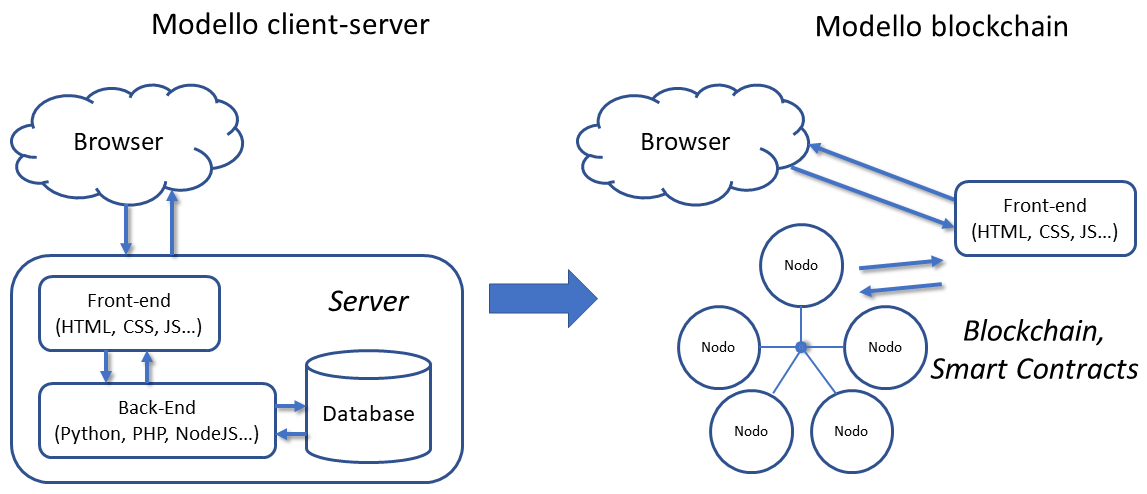
\includegraphics[width=1\textwidth]{immagini/archit.png}
\caption{Architettura Blockchain}
\label{fig:ArchitetturaBlockchain}
\end{figure}

In relazione al classico modello client-server nel modello decentralizzato lo strato back-end è direttamente implementato nella blockchain attraverso gli smart contracts. L’esecuzione della logica dei contratti avviene grazie alla macchina virtuale Ethereum (EVM) eseguita da ciascun nodo della rete estendendo così il concetto di database distribuito con la nozione di calcolo distribuito (distributed computing\footfullcite{wikidistrComp}). Ethereum prevede un meccanismo di incentivi incorporato nel sistema di consenso della rete attraverso l’uso di una criptovaluta chiamata Ether. La logica transazionale (estesa con i smart contracts) in relazione alla complessità di calcoli computazionali è regolata da un costo espresso in unità di Gas corrispondente a una frazione di Ether. Si tratta di un meccanismo grazie al quale è possibile prevenire lo spam dovuto ad esempio all’esecuzione di programmi che non terminano in un tempo finito.

In questo capitolo verranno analizzate queste modifiche ed espansioni della blockchain Ethereum.

\subsection{Transazioni}

Le transazioni in Ethereum sono estese con tre nuove proprietà:

\begin{itemize}
\item Un campo di dati opzionale
\item Un valore Start Gas
\item Un valore Gas Price
\end{itemize}

In riferimento alle transazioni del capitolo precedente (come ad esempio quella in figura \ref{fig:TransazioneToken}) queste proprietà vengono aggiunte ai campi già descritti precedentemente: mittente, destinatario e valore da trasferire. Le nuove proprietà o campi sono strettamente legati al funzionamento della EVM che può accedere ai campi della transazione.

In particolare il campo di dati (opzionale) può essere usato per identificare specifiche operazioni sulla blockchain come ad esempio la registrazione di domini. Prima di andare avanti è opportuno spiegare che Ethereum prevede due tipi di account, quelli appartenenti agli utenti e ai contratti. Questi account posseggono le stesse caratteristiche. Sono identificati da un indirizzo, mantengono il bilancio di token disponibili e così via, funzionano alla stessa maniera con l’eccezione che i primi (account utente) sono controllati da chiavi private (quindi utenti veri e propri) e gli altri dal codice eseguito in maniera automatica. Proprio per la necessità di eseguire programmi equivalenti al codice dei contratti, sono state create le proprietà Start Gas e Gas Price. Start Gas rappresenta il numero massimo di passi (\emph{step}) computazionali che la transazione a cui si riferisce può eseguire. Gas Price, rappresenta il costo che il mittente è disposto a pagare per l’esecuzione dei programmi. Di solito l’incremento di quest’ultima proprietà permette di conquistare una certa priorità nel processo di validazione delle transazioni\footfullcite{ethWhitepaperTx}.

Come già introdotto, i valori Start Gas e Gas Price permettono di rimediare ai problemi relativi all'esecuzione di programmi infiniti e la conseguente congestione della rete dovuta a un numero eccessivo di calcoli computazionali costosi.

\subsection{Patricia Trees}
% --- da migliorare
La struttura dati usata in Ethereum prende il nome di Patricia Tree (o trie) e rappresenta un’estensione di Merkle Tree (per la definizione si rimanda al capitolo 2.3). Se per lo strato concettuale i Merkle Tree servivano fondamentalmente per la memorizzazione e la verifica delle transazioni attraverso procedimenti di hashing ricorsivi, in Ethereum sono usati anche per memorizzare lo stato della rete e il risultato delle transazioni. In particolare in un blocco della rete al posto di una radice di Merkle Tree (tx root), sono incluse le seguenti tre radici di Patricia Tree:

\begin{itemize}
\item Radice dello stato
\item Radice delle transazioni
\item Radice delle ricevute (delle transazioni)
\end{itemize}

Analogamente a quanto detto per i Merkle Trees, in Patricia Trees grazie all'applicazione ricorsiva di funzioni hash crittografiche (in Ethereum viene usato lo standard SHA-3 e in particolare l'algoritmo Keccak256\footfullcite{sha3Wiki}) la radice diventa una sorta di impronta digitale per l'intera struttura dati sottostante. Ogni modifica a qualsiasi livello della struttura farà cambiare il risultato dell'applicazione di funzioni hash sul ramo interessato dalla modifica fino alla radice stessa. 

\begin{figure}[H]
\centering
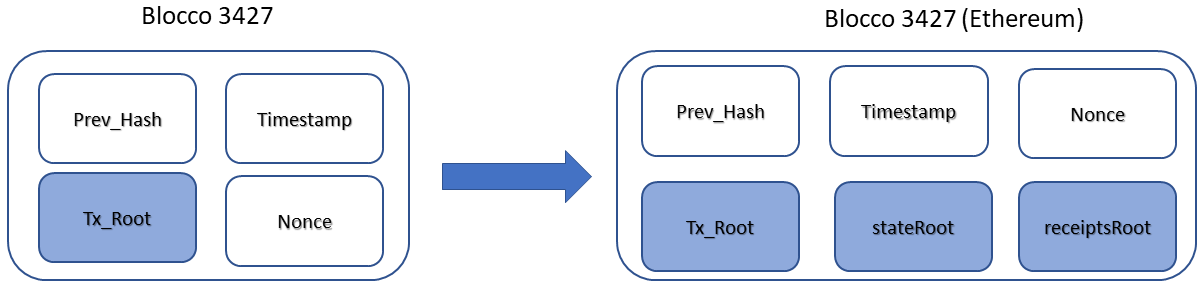
\includegraphics[width=1\textwidth]{immagini/EthBlockSimplified.png}
\caption{Ethereum: Semplificazione blocco}
\label{fig:BloccoEthereumSemplif}
\end{figure}

Dunque in relazione al concetto di blocco illustrato nel capitolo 2.1, la figura \ref{fig:BloccoEthereumSemplif} rappresenta una semplificazione del blocco Ethereum (per la completa lista delle proprietà si rimanda alla sezione 4.3. "The Block" del Yellowpaper Ethereum\footfullcite{ethYellowpaper}).

Un aumento della complessità delle transazioni ha come conseguenza diretta l’espansione dell’intero stato della rete Ethereum. In questa implementazione, per lo stato della rete si intende essenzialmente lo stato di tutti gli account della blockchain (inclusi account esterni e contratti). Lo stato della rete è mutabile a causa della presenza degli smart contracts e deve essere memorizzato perché può cambiare in qualunque momento in seguito all’esecuzione automatica dei contratti. Se la struttura Merkle Tree una volta creata veniva mantenuta in maniera immutabile, in Ethereum è neccessario tenere conto di modifiche frequenti dello stato.

L’altra novità del blocco Ethereum (in figura \ref{fig:BloccoEthereumSemplif}) è la radice delle ricevute. Ogni blocco contiene ricevute permanenti delle transazioni relative al blocco che le contengono.

Patricia Tree facilità l'inserzione, l'eliminazione e l'aggiornamento di dati, obiettivi importanti per questioni di efficienza in una situazione dove lo stato della rete necessita di aggiornamenti frequenti. Infine nelle applicazioni reali permette agli utenti di fare ricerche come ad esempio, trovare una data istanza di un evento X (ad esempio: inserimento di un oggetto nella blockchain) fatta da un utente Y con un certo indirizzo negli ultimi Z giorni.
Per una descrizione formale di questa struttura dati si rimanda all’appendice D, “Modified Merkle Patricia Tree” del Yellowpaper Ethereum\footfullcite{ethYellowpaper}.

\section{Smart Contracts}

Una delle potenzialità più promettenti di Ethereum deriva dall’implementazione di un linguaggio di programmazione Turing completo il quale permette di scrivere contratti (intelligenti) chiamati per l’appunto Smart Contracts. Il termine è stato coniato da Nick Szabo nel 1994 che, lo definisce come un "protocollo di transazione computerizzato che esegue i termini di un contratto\footfullcite{SzaboSmartContract}". Una definizione sempre attuale che nel caso del paradigma soggetto di questa tesi, può essere espressa come contratto o programma immutabile situato direttamente sulla blockchain. Come già detto nella sezione precedente, i contratti fanno parte dello stato della rete e quindi hanno un vero e proprio indirizzo con delle proprietà. Quando vengono soddisfatte certe condizioni descritte nel codice, automaticamente verranno avviate specifiche azioni anch'esse definite nel codice del contratto.

I contratti una volta creati e quindi situati sulla blockchain ereditano le proprietà del paradigma. Sono immutabili, cioè una volta creati non possono essere più modificati, il loro codice è trasparente e quindi consultabile da qualsiasi utente e infine sono distribuiti, il risultato delle azioni compiute nei contratti può essere validato o controllato da tutti.

Queste caratteristiche favoriscono la disintermediazione e potenzialmente la nascita di una situazione dove il codice definito nei contratti diventa l’espressione dei vincoli specificati nelle normative legali. Un esempio significativo dei vantaggi derivati dall'utilizzo di questi contratti può essere fatto analizzando il servizio  di finanziamento collettivo Kickstarter\footfullcite{kickstarter}, basato sull'architettura tradizionale client-server.
\\
\begin{figure}[H]
\centering
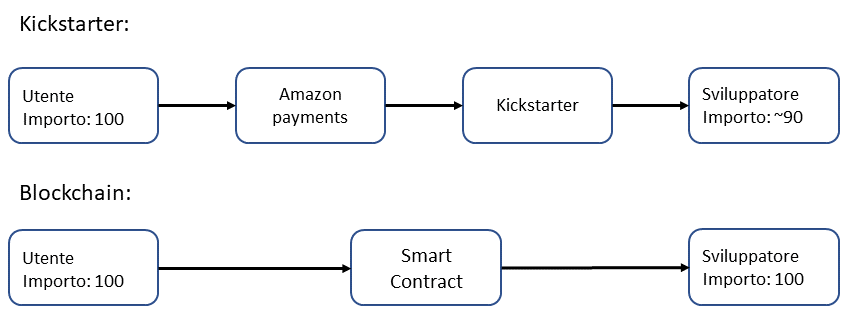
\includegraphics[width=1\textwidth]{immagini/kickstarter.png}
\caption{Ethereum: Esempio Finanziamento Collettivo}
\label{fig:Kickstarter}
\end{figure}

Il procedimento è esemplificato in figura \ref{fig:Kickstarter}, sostenere un progetto con Kickstarter necessita di almeno due intermediari. Il sistema di pagamento Amazon il quale addebita circa 3-5 percento della somma totale e lo stesso servizio Kickstarter che guadagna il cinque per cento dei fondi raccolti. In un'applicazione analoga costruita su Ethereum è possibile fare a meno delle commissioni dovute agli intermediari mantenendo un elevato livello di sicurezza. In entrambi i casi se la raccolta non viene completata entro il termine specificato gli importi verranno restituiti agli utenti. I contratti sostituiscono anche la parte back-end gestita dall'intermediario garantendo che, dopo una certa scadenza definita nel contratto gli importi saranno restituiti agli indirizzi che hanno contributo alla raccolta. 

Importante notare che la scrittura di contratti immutabili deve essere preceduta da un’accurata fase di test automatizzati e simulazioni in modo da individuare eventuali errori e comportamenti non previsti dei programmi che potrebbero avere gravi conseguenze una volta pubblicati sulla rete.

\subsection{Solidity}

Solidity è uno dei principali linguaggi di programmazione orientato alla scrittura dei contratti sulla blockchain\footfullcite{solidity}. Implementato da Ethereum è un linguaggio ad alto livello, fortemente tipato, supporta il meccanismo di eredità e ha una sintassi ispirata a quella di C++, Python e Javascript.
Un contratto Solidity è dunque una collezione di codice incapsulato nelle funzioni e di dati che formano lo stato del contratto (permanentemente memorizzato sulla blockchain) e che risiedono sotto uno specifico indirizzo della blockchain Ethereum.
\\
\begin{lstlisting}[caption={Esempio contratto Solidity},language=JavaScript]
pragma solidity ^0.4.25;

contract storeNum {
  uint256 number;
  address owner;

  modifier onlyOwner { 
    require(msg.sender == owner);
    _;
  }
  
  constructor(uint256 _number) public {
    number = _number;
    owner = msg.sender;
  }

  function changeNum(uint256 _newNumber) public onlyOwner {
    number = _newNumber;
  }
}
\end{lstlisting}

Questo semplice esempio di contratto “storeNum” permette al suo creatore di memorizzare e modificare un numero naturale. Analizzare questo esempio può essere utile per introdurre alcune novità del linguaggio.

\renewcommand\labelitemii{\textbullet}
\begin{itemize}
\item \emph{pragma} (riga 1) definisce la versione del compilatore Solidity da usare per il contratto.
\item \emph{contract storeNum} (righe 3, 5) inizializza il contratto “storeNum” con due variabili di stato: number, può contenere un numero positivo di 256bit e owner che potrà contenere un indirizzo Ethereum di 20byte.
\item \emph{modifier onlyOwner} (righe 7, 10) definisce un insieme di condizioni da applicare a una o più funzioni. Spesso viene usato per definire una guardia di controllo dell'accesso alle specifiche funzioni. In questo caso controlla che l'indirizzo che chiama il contratto sia equivalente a quello di chi lo ha creato.
    \begin{itemize}
        \item \emph{require} è un'istruzione che può creare un'eccezione con il conseguente ripristino dello stato del contratto a quello immediatamente antecedente alla sua chiamata. Require è fondamente per la gestione degli errori in Solidity, è buona regola utilizzarlo il prima possibile per non intercorrere nei costi dovuti all'esecuzione di istruzioni che devono soddisfare certi requisiti oppure possono produrre errori. 
        \item \emph{msg.sender} è un'istruzione predefinita di Solidity, restituisce l'indirizzo che, al momento della chiamata, sta interagendo con il contratto.
        \item {\_}; è un'istruzione specifica dei modifier, stabilisce il punto nel quale viene inserito il corpo della funzione da essa controllata. Dunque, se il flusso di esecuzione del programma non viene interrotto fino a questo punto allora solo adesso verrà eseguito il codice della funzione.
    \end{itemize}
\item \emph{constructor} (righe 12, 15) funziona esattamente come in altri linguaggi, al momento della creazione il contratto viene inizializzato con valori specificati nel costruttore.
\item \emph{changeNum} (righe 17, 19) questa funzione permette di modificare il valore memorizzato nella variabile di stato number. È controllata dal modifier onlyOwner e quindi verrà eseguita solo se viene chiamata dall’indirizzo che ha creato il contratto altrimenti nessun cambiamento di stato verrà effettuato nel contratto. Questa modifica non pregiudica l'immutabilità dei dati, il valore storico della variabile number sarà sempre contenuto nei blocchi precedenti.
\end{itemize}

Un’ultima considerazione sull’esempio del contratto riguarda la visibilità e l’accesso alle funzioni dichiarate. In Solidity le funzioni sono di default pubbliche (\emph{public}) e quindi possono essere chiamate ed eseguite da tutti. Pertanto, è raccomandabile specificare questo parametro nella dichiarazione della funzione stessa. La documentazione già citata prevede parametri tra cui private (solo le funzioni all’interno del contratto in cui sono contenute potranno chiamare questa funzione), view (per funzioni che non cambiano lo stato del contratto) e molte altre. Un modo immediato per provare ed eseguire i contratti (come l'esempio del contratto storeNum di questa sezione) senza la necessità di operare sulla blockchain è quello di usare il compilatore ufficiale Remix\footfullcite{remix} di Ethereum.

Supponendo che il contratto sia corretto e termini in un tempo finito, il passo successivo consiste nella compilazione del codice Solidity in byte-code eseguibile da EVM in maniera simile a come avviene con JAVA e la componente JVM\footfullcite{wikiJVM}.

\subsection{Ethereum Virtual Machine}

Ethereum Virtual Machine o EVM, è una macchina virtuale che viene eseguita da ciascun partecipante della rete Ethereum. I contratti scritti in un linguaggio ad alto livello come ad esempio Solidity sono compilati in byte-code EVM che, nell'insieme rappresenta una sequenza di istruzioni di basso livello chiamate opcode\footfullcite{opcode} eseguibili dalla macchina virtuale. L’esecuzione avviene in modalità protetta (\emph{sandobox}) durante la quale il codice eseguito è isolato, l’EVM (durante il \emph{runtime}) non ha accesso alla rete, ai file locali di sistema o altri processi in esecuzione. A livello della rete tutti gli utenti eseguono in maniera indipendente i calcoli sulla EVM definibile quindi come un computer globale condiviso o \emph{world computer}.

Formalmente la EVM spesso è definita come una macchina quasi Turing completa. Questa affermazione deriva da un’ulteriore vincolo legato al costo computazionale delle istruzioni eseguite al suo interno, misurato in gas, un parametro che limita la quantità di computazione che può essere compiuta durante l’esecuzione\footfullcite{ethYellowpaper}. Ricapitolando a livello dell'implementazione, la EVM assume un ruolo centrale per l'applicazione dei concetti descritti nelle sezioni precedenti. Concetti relativi alle transazioni, al calcolo e consenso distribuito nella blockchain Ethereum.

\subsection{Gas}

Il costo della computazione è rappresentato attraverso Gas, un’unità di misura corrispondente a una frazione di Ether. Gas può essere considerato come una specie di carburante per la EVM, ogni istruzione eseguita al suo interno consumerà una quantità predefinita di Gas. A livello di transazioni l’utente può impostare l’ammontare di Gas che è disposto a spendere per eseguire una certa transazione. In particolare, Gas price indica il prezzo misurato in \emph{gwei}, dove \(10^{9}\) gwei corrispondono a 1 ether cioè 1 ether equivale a 1,000,000,000 gwei\footfullcite{etherUnits}. Il parametro Gas start (in questo contesto chiamato anche Gas limit) impone un limite alla quantità di Gas per la quale l’utente è disposto a pagare il prezzo stabilito.
Infine, il prodotto tra questi due valori, Gas price e Gas start, indica il limite superiore del costo di esecuzione che l’utente vorrebbe spendere così come nel seguente esempio in figura \ref{fig:GasEth}.

\begin{figure}[H]
\centering
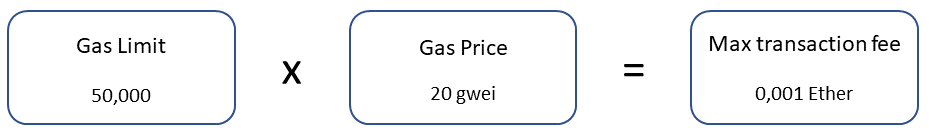
\includegraphics[width=1\textwidth]{immagini/gas.png}
\caption{Gas: Esempio Calcolo Commissioni}
\label{fig:GasEth}
\end{figure}

Le transazioni verranno eseguite dalla EVM finché il programma termina oppure termina la quantità di Gas disponibile per la transazione. Nel caso di una transazione avvenuta con successo al mittente sarà rimborsato il costo di Gas non utilizzato, altrimenti il Gas verrà consumato e la EVM produrrà un'eccezione \emph{out of gas}. Se la quantità di carburante risulta insufficiente per l'esecuzione di una data transazione tutti i cambiamenti effettuati fino a quel punto saranno scartati (ritorno allo stato prima della transazione) mentre il Gas sarà consumato e quindi non verrà restituito al mittente\footfullcite{ethYellowpaper}.

Attenendosi alle condizioni della rete e riguardo i prezzi delle transazioni concluse con successo è possibile fare stime affidabili circa il costo e il tempo di una transazione\footnote{ETH Gas Station (https://ethgasstation.info/) è uno dei siti principali che effettua il monitoraggio dei costi nella rete Ethereum}. Il concetto di Gas è puramente riferito ai calcoli, non è possibile mandare o ricevere unità di Gas, è una misura intesa come una costante con un proprio costo indipendente dalle variazioni di valore di Ether.

\section{Data storage}

Una delle operazioni più costose nelle blockchain è la memorizzazione\footnote{Indicata dall'opcode "SSTORE" contenuto nell'appendice G, “Fee Schedule” di Ethereum Yellowpaper}. Memorizzare in maniera permanente file di grandi dimensioni che, dovranno essere replicati e sincronizzati da tutti i partecipanti della rete implica un costo elevato espresso in termini di Gas. Le blockchain pubbliche, nonostante possano essere definibili come basi di dati distribuite, sono inadeguate per applicazioni che richiedono un uso significativo in termini di spazio di memoria. La regola di base è quella di includere direttamente nelle blockchain soltanto le informazioni, come ad esempio i termini di un contratto, che dovranno godere dei benefici della rete (immutabilità, permanenza, trasparenza ecc.) e memorizzare il resto attraverso servizi esterni.

Tuttavia, è evidente che l'uso di servizi di Cloud Storage tradizionali come AmazonS3, Microsoft Azure o altri sistemi centralizzati limiterebbe i vantaggi delle applicazioni propriamente decentralizzate. Per questo la nascita della tecnologia blockchain è accompagnata dallo sviluppo di sistemi di memorizzazione basate in tutto o in parte sugli stessi principi del paradigma blockchain. Attualmente sono in via di sviluppo molti sistemi di Storage decentralizzato, tra questi i principali Storj\footfullcite{storj}, Sia\footfullcite{sia}, BigchanDB\footfullcite{bigchainDB}, Ethereum Swarm\footfullcite{Swarm} e IPFS\footfullcite{ipfs}.

Questi servizi promettono di usufruire delle novità delle blockchain favorendo la disintermediazione con la conseguente riduzione dei costi dovuti alla memorizzazione di dati e un maggiore controllo su di essi da parte degli utenti finali. In particolare, si è scelto IPFS per lo strato di memorizzazione dell'applicazione decentralizzata che accompagna questo lavoro.

\subsection{IPFS}

IPFS (InterPlanetary File System) è un progetto open-source i cui obiettivi vanno ben oltre l'offerta di un servizio di storage distribuito. Lo scopo principale di IPFS è quello di costruire un file system globale distribuito basato su peer-to-peer in modo da creare una nuova architettura Internet permanente e distribuita. I protocolli alla base di Internet attuale si sono sviluppati secondo livelli di astrazione aggiungendo negli anni via via nuove funzionalità, IPFS costituisce un tentativo di sostituzione e miglioramento di questi protocolli. 

In particolare, riguardo al protocollo di trasmissione HTTP, la differenza sostanziale consiste nel passaggio da un architettura client-server basata su \emph{location based addressing} (indirizzamento in base alla posizione) a un architettura peer-to-peer basata sul \emph{content based addressing} (indirizzamento in base al contenuto). Questo implica una caratteristica importante che può giustificare la scelta di questa particolare tecnologia e la sua integrazione nelle applicazioni blockchain. La caratteristica menzionata riguarda l'indirizzamento delle informazioni in base al contenuto reso possibile grazie all'utilizzo dalle funzioni crittografiche di hash. Memorizzare un dato su IPFS genererà a partire dal contenuto un indirizzo hash che garantisce l'immutabilità del contenuto memorizzato. A livello dell'architettura, l'insieme degli indirizzi IPFS è archiviato attraverso la tabella di hash distribuita, DHT (\emph{Distributed Hash Table}\footfullcite{wikiDHT}). 

\begin{figure}[H]
\centering
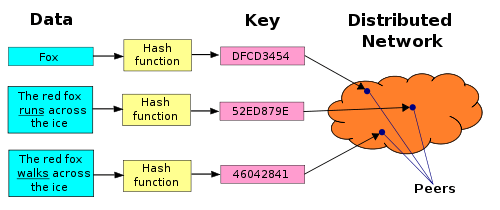
\includegraphics[width=1\textwidth]{immagini/ipfsDHT.PNG}
\caption{IPFS: Indirizzi Hash e DHT}
\label{fig:ipfsDHT}
\end{figure}

Nella figura \ref{fig:ipfsDHT} si può vedere come la chiave (\emph{key}) generata a partire dal contenuto (\emph{data}) entra a far parte della rete distribuita (\emph{DHT}) di cui costituisce un indirizzo univoco. 

Le tecnologie alla base di IPFS sono numerose e la loro descrizione esula dagli scopi di questa tesi, per approfondimenti si rimanda al Whitepaper IPFS\footfullcite{ipfsWhitepaper} che costituisce un punto di riferimento per lo studio della tecnologia. 

La memorizzazione dei dati in maniera distribuita necessita, così come nelle blockchain di un sistema di incentivi. IPFS allo stato dell'arte non ha ancora implementato un meccanismo del genere e dunque non permette di memorizzare dati in maniera permanente. Lo sviluppo della tecnologia mira alla costruzione di un'infrastruttura che, una volta raggiunta una fase stabile permetterà di implementare questo tipo di meccanismi. Filecoin\footfullcite{filecoin} costituisce un esempio di servizio di storage implementato sulla blockchain che potrà essere integrato su IPFS.